%\setchapterimage[6cm]{images/cabecera2}
%\setchapterpreamble[u]{\margintoc}
%%%%%%%%%%%%%%%%%%%%%%%%%%%%%%%%%%%%%%%%%%%%%%%%%%%%%%%%%%%%%

\chapter{Sistemas Punto a Punto}
\label{ch:p2p}
\index{p2p}

\section{Introducción}
Un sistema punto a punto (P2P, peer-to-peer) es un sistema distribuido en el que todos los elementos interconectados tienen el mismo papel
A diferencia del modelo cliente-servidor un sistema P2P proporciona  acceso a recursos de información ubicados en computadores a través de una red.
 

 En \cite{Steinmetz2005} indican que los  sistemas P2P son un sistema autoorganizado de iguales, con entidades autónomas  (pares) que  tiene como objetivo el uso compartido de recursos distribuidos en un entorno en red evitando los servicios centrales.


Es un servicio descentralizado y auto-organizado, con un equilibrio dinámico en  el almacenamiento  y en el procesamiento de recursos de información
En P2P se distribuye las cargas de trabajo entre los equipos participantes, mientras  estos equipos se unen y abandonan el servicio. Esto posibilita el compartir los  datos y recursos a muy gran escala 
 
En los sistemas P2P se  eliminan los servidores y su infraestructura. Esto proporcionar servicios y aplicaciones distribuidas utilizando datos y recursos computacionales disponibles en computadoras personales y estaciones de trabajo en Internet.  Su diseño garantiza que cada usuario proporciona sus recursos al sistema.  Los nodos  tiene las mismas capacidades y responsabilidades.
 
Su correcto funcionamiento no depende de la existencia de cualquier administración centralizada. Estan diseñados para ofrecer un grado limitado de anonimato a los proveedores y usuarios de los recursos. 
 
 \paragraph{Características} 
 \begin{itemize}
 	\item  Su funcionamiento eficiente se basa en su algoritmo para la ubicación de datos y el acceso equilibrado a los mismos. 
 	\item Recursos volátiles: sus propietarios no garantizan que vayan a permanecer encendidos, conectados o libres de fallos 
 	\item No garantiza el acceso a recursos individuales  
 	Puede diseñarse para minimizar la probabilidad de fallo de acceso a un recurso replicado. 
 	\item Puede usar algoritmos de consenso en la replicacion para minimizar fallos (Ejemplo, generales bizantinos)
	
 \end{itemize}
 
 \paragraph{Uso de los sistemas P2P}
 Algunas \'areas donde los sitemas P2P pueden ser de utilidad \cite{Bernstein1985}:
\begin{itemize}
	\item Red web comunitaria. Cualquier grupo con intereses comunes, incluida una familia o aficionados, puede usar listas y un sitio web para crear su propia intranet.
	\item Comercio electrónico. P2P puede agregar nuevas capacidades, incluida la conexión y habilitación de los enlaces de una cadena de suministro,
	distribuir información, contenido o software de manera más eficaz y mantener los elementos de información en su nodo original
	 con un directorio central o una capacidad de búsqueda.
	\item  Juegos. Una infraestructura P2P proporciona una base natural para el desarrollo de juegos comunitarios en línea 	que no están controlados centralmente. Los desarrolladores pueden centrarse en las características del juego en lugar de la interfaz del 	protocolo de comunicaciones.
	\item  Los motores de búsqueda. Se puede encontrar información fresca y actualizada buscando directamente en el espacio donde resida el elemento deseado.
	\item  Protección contra el virus. Las relaciones entre los nodos de la comunidad P2P permiten la colaboración en la detección y advertencia de virus, así como la cuarentena automática de la comunidad contra nuevos ataques
	\item Servicios dadicionales. Hay casos en los que es deseable colocar los datos más cerca del cliente que los solicita. Los módulos de capacitación en línea que contienen segmentos de video, por ejemplo, brindan el efecto deseado cuando los archivos de datos grandes se encuentran cerca del alumno en línea. Múltiples clientes que ofrecen espacio de almacenamiento pueden brindar un servicio más flexible y confiable en comparación con un servidor.
	\item  Desarrollo colaborativo. El alcance puede variar desde el desarrollo de productos de software hasta la redacción de un documento.
	a aplicaciones como renderizar gráficos.
\end{itemize}


\paragraph{sistemas P2P no estructurado y estructurado}
	\index{P2P no estructurados}
		\index{P2P estructurados}

Entre los principales retos \cite{Steinmetz2005} de los sistemas P2P radica en la autoorganización descentralizada de un sistema distribuido y en lograr un alto nivel de calidad de servicio sin necesidad de servicios centralizados. Hay dos enfoques principales que se han desarrollado para resolver este problema: sistemas P2P no estructurado y estructurado:

\begin{itemize}
	\item sistemas P2P no estructurados:
	
	Las primeras aplicaciones para compartir archivos basadas en P2P   usaban los llamados enfoques no estructurados. En este enfoque los  sistemas dependían de búsquedas a través de un servidor central que almacenaba las ubicaciones de todos los elementos de datos. Solo después de buscar la ubicación de un elemento de datos a través del servidor, los datos se transfirieron directamente entre pares. Otras implementaciones usan algoritmos de  inundación (ver algoritmos de  inundación en cap. \ref{ch:Comunicación Indirecta} en secci\'on \ref{alg-inun} ).
	Este enfoque tiene como desventaja la dificultad en escalamiento, además de ser un cuello de botella con respecto a recursos como la memoria, la potencia de procesamiento y el ancho de banda, mientras que los enfoques basados en inundaciones muestran un enorme consumo de ancho de banda en la red.  
	
	\item sistemas P2P estructurados: \index{tablas hash distribuidas}
	Este enfoque estructurado esta basado en \gls{tablas hash distribuidas}, DHT (DHT, Distributed Hash Table).  Son un tipo de tablas hash que almacenan pares  clave-valor y permiten consultar el valor asociado a una clave, donde   los datos se almacenan de forma distribuida en   nodos  y proveen un servicio eficiente de búsqueda que permite encontrar el valor asociado a una clave.
	
    Las tablas hash distribuidas (DHT)  \cite{Wehrle2005a}  proporcionan una estructura de indexación distribuidas, es decir, el  almacenamiento de datos distribuidos y direccionables por contenido; así como    escalabilidad, confiabilidad y tolerancia a fallos. Por lo general, un elemento de datos se puede recuperar de la red con una complejidad de $O(logN)$. De igual manera,  agregar nuevo contenido o pares a la red  y manejar fallas, 	comúnmente tienen una complejidad de $O(logN)$ y $O(log_{2}N)$, respectivamente.
 
\end{itemize}

 \section{Evoluci\'on de los sistemas P2P}
 \index{P2P!evoluci\'on}
La evoluci\'on de los sistemas P2P tambi\'en se pueden estudiar desde el punto de vista de las generaciones. A saber, hay tres generaciones, la 1era generaci\'on basada en servicios de intercambio de m\'usica como Napster; la 2da generaci\'on en aplicaciones de archivos compartidos, por ejemplo Freenet \cite{Clarke2001}, Gnutella, Kazaa \cite{Leibowitz2003}, BitTorrent \cite{Cohen2003}; y la 3era generaci\'on basado en tablas hash distribuidas, como  Pastry  \cite{Rowstron2001}, Tapestry   \cite{Zhao2001}, 
CAN  \cite{Ratnasamy2001}, Chord   \cite{Stoica2001} y Kademlia  \cite{Maymounkov2002}.



 \subsection{ 1-era Generación: Napster}  
  	\index{P2P!1era generacion} \index{Napster}  	
  	
 Napster fue una aplicación para compartir archivos entre pares que se lanzó escrita  por Shawn Fanning \cite{Eberspaecher2005}  y se lanz\'o el 1 de junio de 1999 con énfasis en la distribución de archivos de audio digital. Las canciones de audio compartidas en el servicio generalmente se codificaban en formato MP3.  A medida que el software se hizo popular, la empresa se encontró con dificultades legales por la infracción de los derechos de autor. Cesó sus operaciones en 2001 después de perder una ola de juicios y se declaró en quiebra en junio de 2002 \cite{Coulouris2011} 	\cite{Eberspaecher2005} \cite{Eberspaecher2005a}.
 
 La arquitetura de Napster se centra en un servidor central o  
 servidor de indices , ver Figura \ref{fig:napster} que contenian los 
 Indices unificados para cada archivo.  
 El modo de operaci\'on de Napster era de la siguiente manera:
 
 \begin{enumerate}
 	\item El usuario accede al servidor de \'indices para buscar la ubicaci\'on del archivo solicitado.
 	\item El archivo de \'indices proporciona al usuario una lista de nodo que contiene ese archivo.
 	\item El usuario  hace la solicitud directa  del archivo a un nodo seleccionado de la lista proporcionada. 
 	\item El nodo que contiene el archivo le proporciona al usuario al archivo seleccionado.
 	\item Posteriormente, el nodo que obtuvo el archivo nuevo pasa a formar parte de la lista \'indices del servidor como un poseedor del archivo.
 \end{enumerate}
 
 Napster aprovechó las características especiales de la aplicación, como que los archivos de música nunca se actualizan y no se requieren garantías con respecto a la disponibilidad de archivos individuales.
 La ventaja de los sistemas centralizados es que son simples de implementar y localizan los archivos de manera rápida y eficiente.
 Su principal desventaja es que son vulnerables a la censura, acciones legales, vigilancia, ataques maliciosos y fallas técnicas, ya que el contenido compartido, o al menos las descripciones del mismo y la capacidad de acceder a él, están controlados por una sola institución, empresa o usuario. 
 
 Napster utilizó un índice unificado (replicado) de todos los archivos de música disponibles.  Es probable que el descubrimiento y el direccionamiento de objetos ocasionaran  cuellos de botella. 
  Adem\'as la coherencia entre las réplicas no era fuerte. Estos sistemas se consideran intrínsecamente no escalables, ya que seguramente habrá limitaciones en el tamaño de la base de datos del servidor y su capacidad para responder a las consultas y la dificultad de mantener requisitos de consistencia minimos.
 

 \begin{figure}%
 			\begin{center}
 	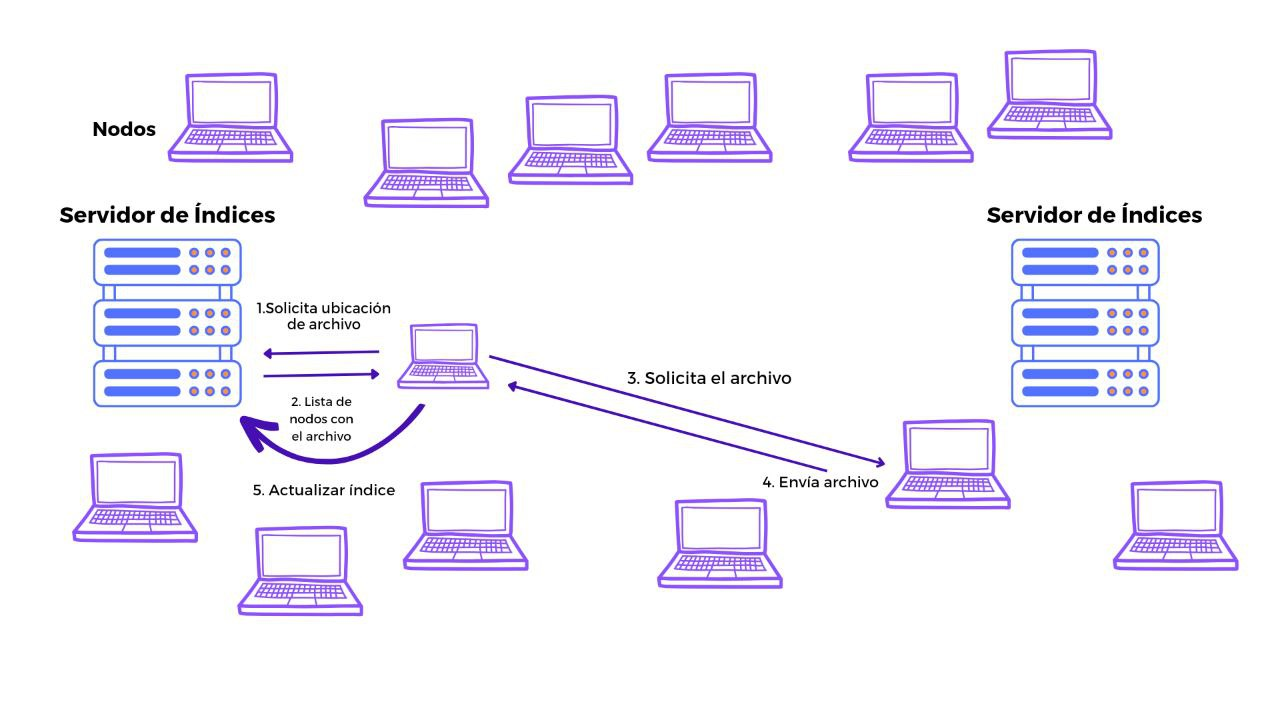
\includegraphics [width=0.8\linewidth]{10/1.jpg } 
 	\caption{Arquitectura de Napster}
 	\label{fig:napster}
 			\end{center}
 \end{figure}

 
 
 \subsection{2-da Generación. Gnutella}
 
 \index{P2P!2da generacion} \index{Gnutella}
 
 En Gnutella como enfoque no estructurado, no hay un control general sobre la topología o la ubicación de los objetos dentro de la  red. No existe una coordinación central de las actividades de la red.
 Los usuarios se conectan entre sí directamente de forma \textit{ad hoc} a través de una aplicación de software \cite{Eberspaecher2005a} \cite{Buford2009}.
 
 \paragraph{Similitudes entre Gnutella y Napster}
 \begin{itemize}
 	\item  Los usuarios colocan los archivos que desean compartir en sus discos duros y los ponen a disposición  a todos los demás para descargarlos de igual a igual.
 	\item Los usuarios ejecutan una parte del software Gnutella para conectarse a la red Gnutella.
 \end{itemize}
 
 \paragraph{Diferencias entre Gnutella y Napster}
 \begin{itemize}
 	\item No existe una base de datos central que conozca todos los archivos disponibles en la red Gnutella. En cambio, todas las máquinas de la red se informan entre sí sobre los archivos disponibles mediante un enfoque de consulta distribuida.
 	\item Hay muchas aplicaciones cliente diferentes disponibles para acceder a la red Gnutella.
 \end{itemize}
 
 \paragraph{Arquitectura de Gnutella}
 
 En la Figura \ref{fig:gnutella} se muestra un esquema de la arquitectura Gnutella.
 Los nodos son iguales al resto de los nodos pero algunos ofrecen otro servicio. 
 Los \textbf{Ultrapeers} son  algunos nodos son designados para tener recursos adicionales
 Las \textbf{hojas}  se conectan a un pequeño número de ultrapeers que están fuertemente conectados a otros nodo (con más de 32 conexiones cada uno).
 Esto reduce el número máximo de saltos para una búsqueda exhaustiva.
 
 Este estilo de arquitectura se conoce como  arquitectura híbrida y es el enfoque adoptado en Skype (ver cap. \ref{ch:Pro-Hil} en secci\'on \ref{Skype}).
 
 
 
  La estrategia de b\'usqueda que usa Gnutella se basa en lo siguiente. 
 \begin{enumerate}
 	\item El nodo solicitante inicia la búsqueda del archivo A
 	\item  Envía mensaje a todos los nodos vecinos solicitando el archivo A
 	\item  En caso de no tener la ubicaci\'on del archivo A, los vecinos reenvían el mensaje al resto de sus vecinos en la red.
 	\item  Los nodos que tienen el archivo A inician un 	mensaje de respuesta
 	\item El mensaje de respuesta a la consulta se propaga hacia atrás hasta el nodo solicitante
 	\item  Con la ubicaci\'on conocida, se descarga el archivo A.
 \end{enumerate} 
 
  Las hojas y los  ultrapeers utilizan el Protocolo de enrutamiento de consultas (QRP, Query Request Protocol) para intercambiar una tabla de enrutamiento de consultas (QRT, Query Routing Table ). El QRT consta de una tabla de palabras clave hash que los nodo hoja envía a sus ultrapeers.
   Un nodo hoja envía su QRT a cada uno de los ultrapeers a los que está conectado, y los ultrapeers fusionan el QRT de todas sus hojas  más su propio QRT (si comparten archivos) y lo intercambian con el suyo propio.   Luego, el enrutamiento de consultas se realiza mediante el hash de las palabras de la consulta y viendo si todas coinciden en el QRT. Los ultrapeers hacen esa verificación antes de reenviar una consulta a un nodo hoja y también antes de reenviar la consulta a un ultrapeers del mismo nivel, siempre que este sea el último salto que la consulta puede realizar.
 
 
 El protocolo  QRP fue diseñado para reducir el número de consultas emitidas por nodos.  El protocolo  se basa en el intercambio de información sobre los archivos contenidos en los nodos y solo reenvía las consultas por rutas donde el sistema cree que habrá un resultado positivo.
 En lugar de compartir información sobre archivos directamente, el protocolo produce un conjunto de números hash en las palabras individuales a partir de un nombre de archivo.
  El protocolo QRP Gnutella versión 0.4 emplea estos tipos de mensaje:
  
 \begin{itemize}
 		\item Mensajes de difusión:  		
 		\begin{itemize}
 			\item  Ping: mensaje de inicio 
 			\item Consulta: patrón de búsqueda y TTL (time-to-live)  
 		\end{itemize}
 		
 			\item Mensajes de retropropagaci\'on: 
 				\begin{itemize}
 				\item Pong: responde a un ping, contiene información sobre el par.
 				\item Respuesta a la consulta: contiene información sobre la computadora.
 				que tiene el archivo necesario
 			\end{itemize}
 			
 			
 			\item Mensajes de nodo a nodo: con protocolo HTTP 
 			\begin{itemize}
 				\item GET: devolver el archivo solicitado
 				\item PUSH: envíame el archivo
 			\end{itemize}
 \end{itemize}

 
 	 
   
  	
  	\begin{figure}%
  				\begin{center}
  			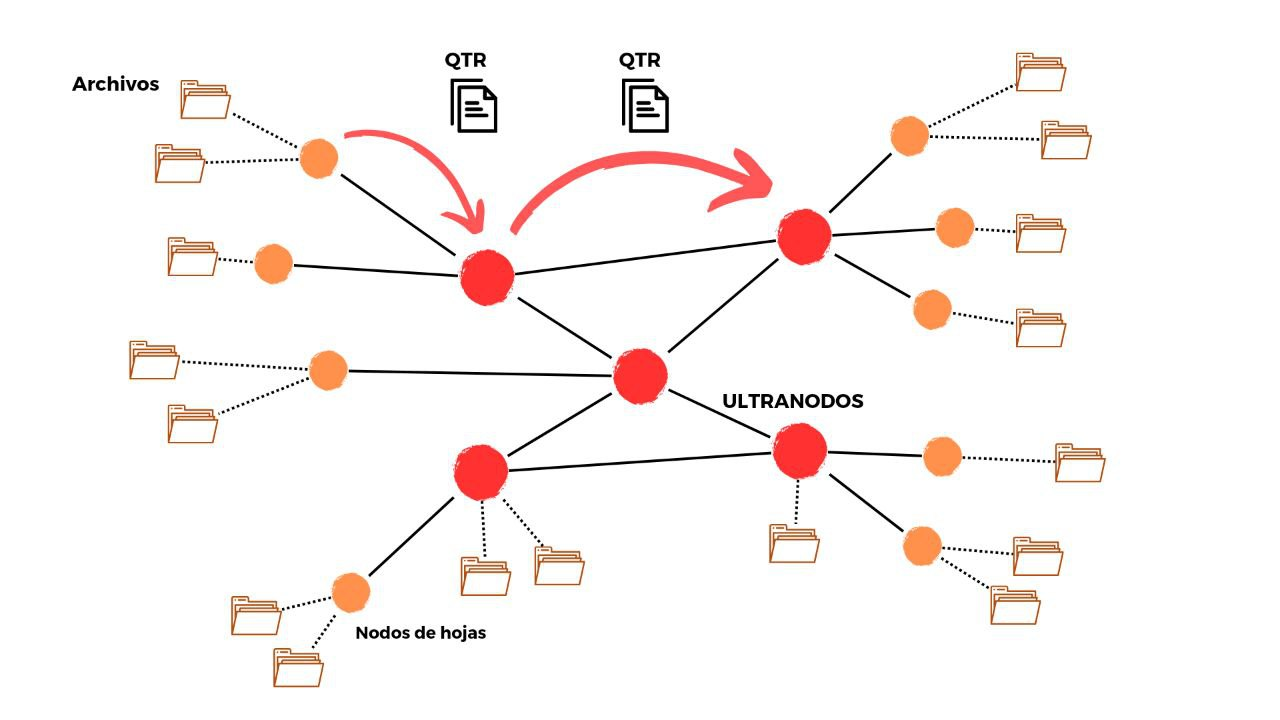
\includegraphics[width=0.8\linewidth] {10/2.jpg } 
  		\caption{Arquitectura de Gnutella}
  		\label{fig:gnutella}
  				\end{center}
  	\end{figure}
 
 \subsection{3-era Generación. Algoritmos DHT}  
 \index{P2P!3era generacion} \index{algoritmos DHT}

 
%%\cite{Eberspaecher2005a}  Pastry  \cite{Rowstron2001}, Tapestry   \cite{Zhao2001},  CAN  \cite{Ratnasamy2001}, Chord   \cite{Stoica2001} y Kademlia  \cite{Maymounkov2002}
 
 
 
 \subsubsection{Chord}
 \index{Chord}
 
 Chord  \cite{Stoica2001}  \cite{Goetz2005} \cite{Wehrle2005a} es un protocolo de búsqueda y un algoritmo para tablas hash distribuidas estructuradas.  Los nodos están organizados lógicamente  en un anillo de tal forma que un elemento de datos con llave $k$ se mapea hacia el nodo con  el identificador más pequeño $id \geq k$. El nodo se conoce como sucesor de la clave $k$, y se denota  como $succ(k)$.
 
 La Figura   \ref{fig:chord-te} muestra un círculo de identificadores inicializado con $n = 6$, es decir, $2^{6} = 64$ identificadores, diez nodos y siete elementos de datos. El sucesor de la clave $K5$, es decir,
 el nodo contiguo en el sentido de las agujas del reloj es el nodo N8, donde se encuentra K5. El sucesor de K43 es N43 ya que sus identificadores son iguales. La estructura circular módulo $2^{6} = 64$  da como resultado que K61 esté ubicado en N8
 
  
 \paragraph{Espacio Chord}
 El espacio de nodos en Chord se considera circular, lo que significa que entre los nodos ubicados entre los identificadores  $0$ y $2^n-1$ se consideran nodos vecinos.La distancia entre dos nodos se basa en las direcciones. Para calcular esta distancia  Chord utiliza la diferencia numérica entre los dos identificadores o  GUID  (GUID, Global Unique Identifier) como distancia. 

 Noten que la  distancia calculada del nodo A al nodo B no es la misma que la distancia calculada del nodo B al nodo A. El cálculo de la distancia entre un nodo A y un nodo B varía dependiendo de si el GUID de A es mayor o menor que el GUID de B:
 
 \begin{itemize}
 	\item  Si \quad $GUID  \,  A  \leq GUID \,   B$, entonces $dist(A, B) = GUID \,  B - GUID \,  A$
 	
 	\item Si \quad $GUID \,  A  \geq GUID \,  B$, entonces $dist(A, B) = GUID \,  B + 2^n - GUID \, A $
 \end{itemize}
 
 
 \paragraph{Tablas de enrutamiento}
 
 Para que los pares en una red Chord puedan encontrarse entre sí, cada par necesita conocer  la dirección IP   de su vecino más cercano en términos de los  GUID de los nodos en la red Chord.  
Con sólo conocer el par vecino más cercano en la red es posible encontrar cualquier par en la red. El algoritmo de búsqueda de Chrod  se detalla a continuaci\'on:
 

\begin{enumerate}
	\item  Si el vecino más cercano es el par GUID que está buscando, la búsqueda finalizó exitosamente.
	
	\item De lo contrario, solicite al vecino más cercano que le devuelva la dirección del par que está buscando o el par más cercano que conoce al par objetivo, si el vecino no conoce al par objetivo:
	\begin{enumerate}
		\item Si el par devuelto GUID es el par que está buscando, la búsqueda finalizó correctamente.
		
		\item Si el par vecino no conoce a ningún par más cercano al par objetivo que él mismo, no devuelve información del par. La búsqueda finaliza sin éxito.
	\end{enumerate}	
	
	\item De lo contrario, repita 2) pero envíe la solicitud al par que acaba de recibir de la solicitud de búsqueda anterior.
	
\end{enumerate}

	
La búsqueda de pares eventualmente preguntará a todos los pares en la red, uno a la vez, hasta que se encuentre el par que busca, o el último par diga que el par más cercano que conoce al par objetivo es el par que busca en el mismo por de origen, es decir, después de una ronda completa en la red.
Entonces el tiempo de búsqueda es de $O(N)$, lo que significa que el tiempo de búsqueda crecerá linealmente con la cantidad de pares en la red Chord.  

Para mejorar el tiempo de búsqueda, en la tabla de enrutamiento de Chord se mantiene referencias a pares que están exponencialmente cada vez más distantes según su distancia GUID del nodo de referencia. Primero, la tabla de enrutamiento contendrá una referencia al vecino cercano  con una distancia GUID de 1. Luego, una referencia al par con una distancia GUID de $2,  4,  8,  16$, y as\'i. usando la distancia exponencial de $2^{n}$.

 Por   ejemplo en la Figura \ref{fig:chord-te}, en el nodo $n$, la entrada de la tabla en la fila $i$ identifica el primer nodo que sucede a n por al menos $2^{n}-1$, es decir, $succ(n + 2^{n}-1)$, donde $1 \leq i \leq l$. El segundo apuntador del nodo N8 ($8+2^{1}= 10$) es el nodo N10 y el tercer dedo ($8+2^{2}= 12$)   es el nodo N15. 


\begin{figure}%
			\begin{center}
		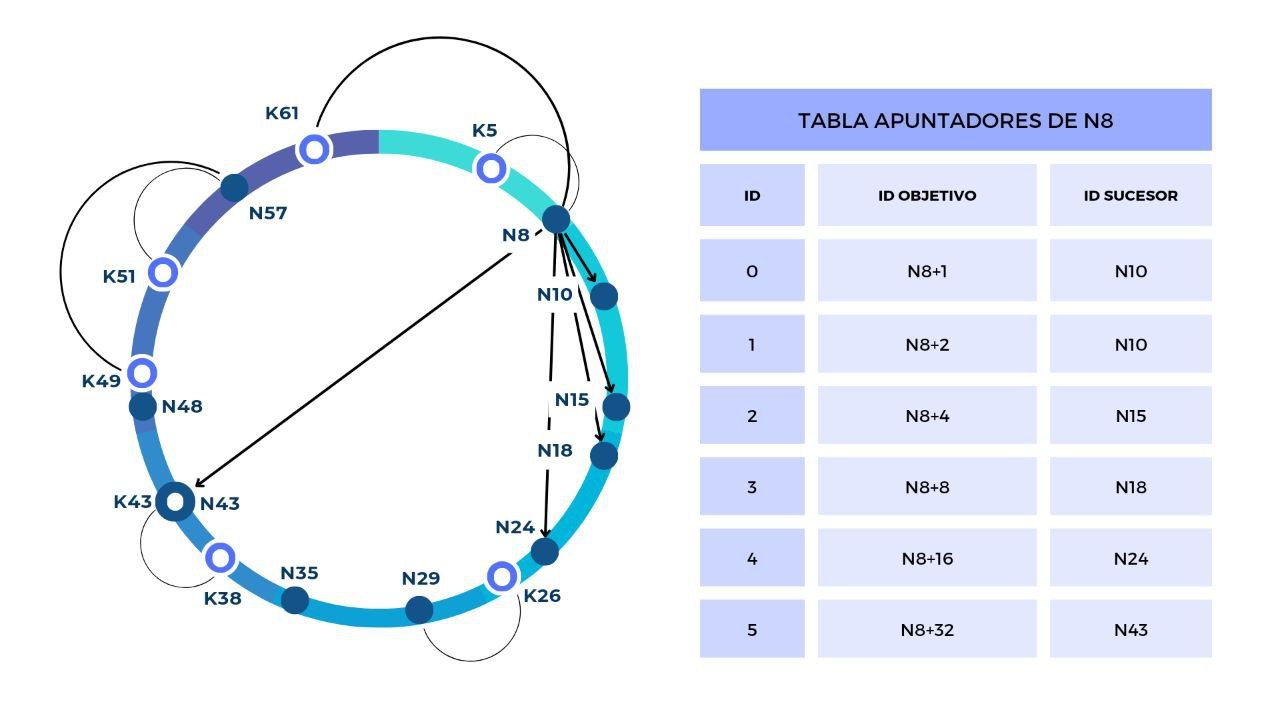
\includegraphics[width=0.8\linewidth] {10/3.jpg } 
	\caption{Tabla de enrutamiento Chord de 6 bits}
	\label{fig:chord-te}. Adaptado de \cite{Goetz2005}
			\end{center}
\end{figure}
 
 Las líneas de puntos indican qué nodos albergan qué claves. Las líneas negras representan a quien apunta el nodo N8.

\paragraph{Protocolo Chord}
El protocolo Chord asigna a cada dirección IP del nodo y clave de archivo un identificador mediante hash consistente. Esos identificadores están ordenados en un anillo de números del $0$ hasta $(2^{n})-1$,  donde $n$ es un número elegido por quien inicia la red Chord P2P. El uso de $n = 8$ daría como resultado que los GUID de acordes vayan de 0 a 255. Los valores n comunes son 64, 128, 160 y más; esto depende de lo que se espera qusean el n\'umero de nodos que se unan a la red de manera que cada nodo pueda obtener n id \'unico. 
  
  

La asignación de claves para un nodo se realiza de la siguiente manera:

\begin{itemize}
	\item Al asignar la clave $K$ a un nodo cuál sería el primer nodo cuyo identificador es igual a $K$  en el espacio de identificadores.
	\item El nodo sucesor de una K (tecla a) es el primer nodo que encontró en el sentido de las agujas del reloj desde K en el anillo de acordes.
	por ejemplo: sucesor(2) = 3
	cuando un par ingresa al ring, ciertas claves que fueron asignadas al sucesor ahora se asignan a un nuevo par
	Cuando un par sale, las claves que fueron asignadas al par saliente ahora se asignan al sucesor
\end{itemize}


 

\paragraph{Tabla de enrutamiento Chord}

 Cuando un nodo quiere unirse al sistema, comienza por generar un identificador aleatorio, id. Observe que si el espacio identificador es lo suficientemente
grande, entonces proporcionar el generador del número aleatorio es de buena calidad; la probabilidad de generar un identificador que ya está asignado a un nodo real es cercana a cero.
Entonces, el nodo puede simplemente realizar la búsqueda en un id, lo cual devolverá la dirección de la red de $succ(_{id})$. En ese punto, el nodo de unión puede simplemente contactar a  $succ(_{id})$ y a su predecesor, e insertarse él mismo en el anillo. Desde luego, este esquema requiere que cada nodo también almacene información sobre su predecesor. La inserción provoca además que cada elemento de datos, cuya llave está ahora asociada con el nodo id, sea transferido desde  $succ(_{id})$.
En términos sencillos: el id del nodo informa su punto de inicio a su predecesor y a su sucesor, y transfiere sus elementos de datos a  $succ(_{id})$.

 \section{Caso de Estudio. Pastry}
\index{Pastry} \index{caso de estudio!Pastry}

 Pastry desarrollado en el año 2001 por los investigadores de Microsoft Research, Antony Rowstron y Peter Druschel \cite{Rowstron2001}.   Se trata de un protocolo que se define como un sistema P2P, completamente descentralizado, escalable y autoorganizado. Emplea un protocolo de transporte UDP en la mayoría de los casos.

  Los nodos de Pastry forman una red superpuesta descentralizada, autoorganizada y tolerante a fallos dentro de Internet. Pastry proporciona enrutamiento de solicitudes eficiente, ubicación determinista de objetos y equilibrio de carga de manera independiente de la aplicación. Además, Pastry tiene mecanismos que admiten y facilitan la replicación de objetos, el almacenamiento en caché y la recuperación de fallas de aplicaciones específicas \cite{Goetz2005}. 
  
Cada nodo en la red Pastry tiene un identificador único global, GUID  (GUID, Global Unique Identifier)   en un espacio de identificador circular de 128 bits. Se supone que el identicador del nodo se genera aleatoriamente y que cada GUID tiene la misma probabilidad de ser elegido. Un nodo con un GUID similar puede estar geográficamente lejos.
 Dada una clave, PASTRY puede entregar un mensaje al nodo con el GUID más cercano a la clave dentro de   $log_{2^{b}}N$ pasos, donde $b$ es un parámetro de configuración (normalmente $b = 4$) y $N$ es el número de nodos de Pastry activos en la red superpuesta.
 
 Supongamos que queremos encontrar el nodo en la red PASTRY con el GUID más cercano a una clave determinada. Tenga en cuenta que GUID y la clave son secuencias de 128 bits. Tanto el GUID como la clave pueden considerarse como una secuencia de dígitos con base $2^{b}$.

% Cuando se le presenta un mensaje y una clave numérica de 128 bits, un nodo Pastry enruta eficientemente el mensaje al nodo con un nodeId numéricamente más cercano a la clave, entre todos los nodos Pastry activos actualmente.

Cada nodo PASTRY tiene un estado que consta de:
\begin{itemize}
	\item una tabla de enrutamiento utilizada en la primera fase del enrutamiento (largas distancias).
	\item conjunto de vecindad $M$ contiene el GUID y las direcciones IP de los nodos en  $|M|$ más cercanos (según una métrica) al nodo considerado. 
	\item un conjunto de hojas $L$ contiene el GUID y las direcciones IP de los nodos en  $|L|/2$ cuyos GUID son numéricamente más cercanos y más pequeños que el GUID actual, y los nodos $|L|/2$ cuyos GUID son numéricamente más cercano y mayor que el GUID actual.
\end{itemize}  



	\begin{figure}%
				\begin{center}
 		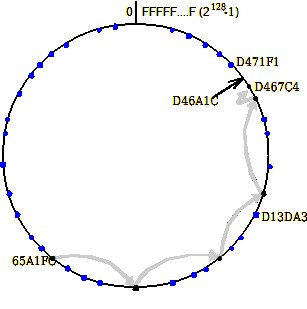
\includegraphics[width=0.8\linewidth] {10/pastry-et} 
		\caption{Anillo Pastry. Tomado de \cite{Coulouris2011}}
		\label{fig:pastry}
				\end{center}
\end{figure}
 
 
 \subsubsection{Tabla de enrutamiento}
 

 
 \subsubsection{Enrutamiento circular}
  
 Un paquete se puede enrutar a cualquier dirección en el espacio de claves, ya sea que haya un nodo con ese GUID de nodo o no, ver Figura \ref{fig:pastry}. Cada hoja contiene un par GUID y direcci\'on IP. 
  El paquete se enruta hacia su lugar adecuado en el anillo circular y el par cuyo GUID esté más cercano al destino deseado recibirá el paquete. El destino m\'as cercano es  un  nodo cuyo NodeId comparte con la clave un prefijo que es al menos un dígito más largo que el que la clave comparte con el nodo actual. 
   Si no se conoce dicho nodo, el mensaje se reenvía a un nodo que comparte el mismo prefijo del nodo real, pero su NodeId está numéricamente más cerca de la clave.
 
% Cada vez que un par recibe un paquete para enrutar o quiere enviar un paquete, primero examina su conjunto de hojas y lo enruta directamente al nodo correcto si encuentra uno
 % El paquete se enruta hacia su lugar adecuado en el anillo circular y el par cuyo GUID esté más cercano al destino deseado recibirá el paquete. 
 
 \subsubsection{Tabla de enrutamiento  }
  La tabla de enrutamiento es una tabla $log_{2^{b}}(N) x (2^{b} - 1)$  donde $b$ es el parámetro de configuración y $N$ es el número de nodos PASTRY en la red.
 Las  $(2^{b} - 1)$ entradas en la fila $n$ cada una se refiere a un nodo cuyo GUID comparte el presente nodo GUID en los primeros $n$ dígitos  pero cuyo $(n + 1)$ésimo dígito tiene uno de los $(2^{b} - 1)$ posibles  valores distintos del $(n + 1)$ésimo dígito en la identificación del nodo actual. Ejemplo de un tabla de enrutamiento esta en la  Figura \ref{fig:pastry-te}. 
 
  Si el enrutamiento circular  falla en la b\'usqueda del par, entonces el par consulta a continuación su tabla de enrutamiento con el objetivo de encontrar la dirección del par que comparte un prefijo del GUID  más largo con la dirección de destino del propio par buscado. Si no existe, elegirá un par de su lista de contactos con el mismo prefijo de longitud cuyo GUID de nodo esté numéricamente más cerca del destino y enviará el paquete a ese par. Dado que el número de dígitos correctos en la dirección siempre aumenta o permanece igual (y si permanece igual, la distancia entre el paquete y su destino se reduce), el protocolo de enrutamiento converge.
  
 M\'as en detalle, para manejar un mensaje $M$ que se diriga  a un nodo $D$ (donde $R[p ,i]$ es el elemento en la columna $i$,   fila $p$ de la tabla de enrutamiento) el algoritmo de b\'usqueda:

 
 
 \begin{enumerate}
 	\item  Si $L_{-{|L|/2}}  \le D \le L_{+{|L|/2}}m$  (//establece si  el destino está dentro de la hoja,  o  es el nodo  actual).
 	\item Dirigir  $M$  al elemento de $Li$ de la hoja de conjunto con GUID más     cercano a D o  al nodo actual A.    
	\item  else  (// usa  la tabla de enrutamiento para despachar M a un nodo con un GUID cercano)
 	\item Búsqueda p, la longitud del prefijo común más larga de D y A, i , el ($p+1$)esimo  dígito hexadecimal de D.
	\item  Si $(R[p, i] \neq nulo)$ dirigir M hacia $R[p,i]$ (// enrutar M a un nodo con el  prefijo común  más largo).
	\item else (// no hay ninguna entrada en la tabla de enrutamiento)
 	\item Avance $M$ a cualquier nodo en $L$ o $R$ con un prefijo común de longitud $p$  con  una GUID que es numéricamente más cerca 
  \end{enumerate}
 
 
 Dado un mensaje, el nodo primero verifica si la clave se encuentra dentro del rango de nodeIds cubiertos por su conjunto de hojas (línea 1). Si es así, el mensaje se reenvía directamente al  nodo de destino, es decir, el nodo en el conjunto de hojas cuyo GUID está más cerca de la clave (posiblemente el nodo actual) (línea 3).
 Si la clave no está cubierta por el conjunto de hojas, entonces se utiliza la tabla de enrutamiento y el mensaje se reenvía a un nodo que comparte un prefijo común con la clave en al menos un dígito más (líneas 6 a 8). En ciertos casos, es posible que la entrada apropiada en la tabla de enrutamiento esté vacía o que no se pueda acceder al nodo asociado (líneas 11 a 14), en cuyo caso el mensaje se reenvía a un nodo que comparte un prefijo con la clave al menos siempre que el nodo local, y esté numéricamente más cerca de la clave que el nodo actual.
 
 %Por ejemplo, un nodo con una tabla de enrutamiento como en la de la Figura \ref{fig:pastry-te} enviaría una  consulta la clave 103200 en el nodo 103210, ya que es el nodo del conjunto de hojas más cercano a    la clave. Dado que el conjunto de hojas contiene los nodos más cercanos, se sabe que la clave está ubicada en ese nodo. Una consulta para la clave 102022, aunque numéricamente más cercana al nodo 101203, se reenvía al nodo 102303 ya que comparte el prefijo 102 con la clave (en contraste con 10 como lo hace el nodo actual). Para la clave 103000, no hay  ninguna entrada en la tabla de enrutamiento con un prefijo común más largo que el nodo actual.
% Por lo tanto, el nodo actual enruta la consulta al nodo 103112 que tiene el mismo  prefijo común 103 pero está numéricamente más cerca que el nodo actual.  Este esquema garantiza que no se produzcan bucles de enrutamiento porque la consulta se enruta estrictamente a un nodo con un prefijo de identificador común más largo que el nodo actual, o a un nodo numéricamente más cercano con el mismo prefijo.
 

  
  	\begin{figure}%
  				\begin{center}
  	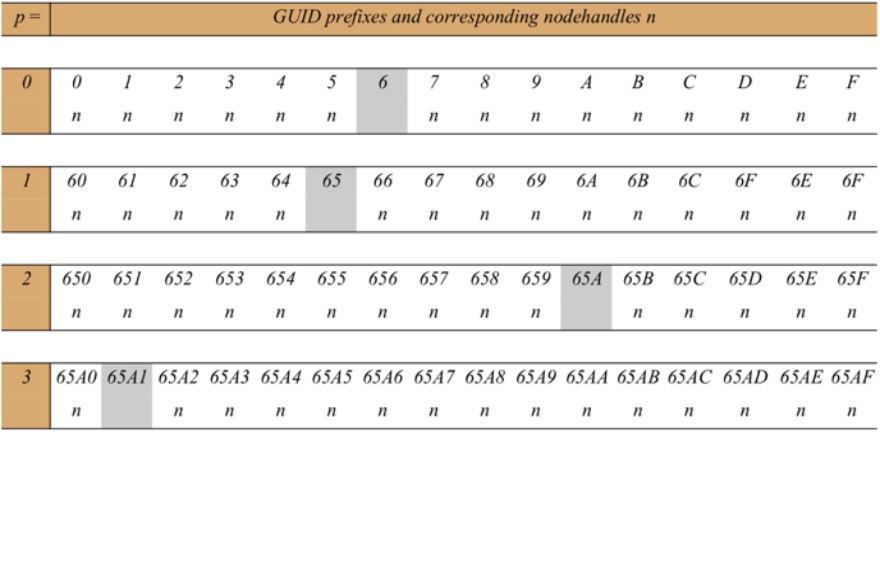
\includegraphics[width=0.8\linewidth] {10/pastry-tab} 
  	\caption{Tabla de enruamiento Pastry. Tomado de \cite{Coulouris2011}}
  	\label{fig:pastry-te}
  			\end{center}
  \end{figure}
 
 
%  En la Figura \ref{fig:pastry-te} Para manejar un mensaje $M$ se dirigió a un nodo $D$ (donde $R[p ,i]$ es el elemento en la columna $i$,   fila $p$ de la tabla de enrutamiento): 
% $R^{i}_{l}$: la entrada en la tabla de enrutamiento $R$ en la columna $i$, $0 \leq i \le 2^{b} $.  y fila l, 0 l < b128=bc. Li: el i-ésimo nodoId más cercano en el conjunto de hojas L, bjLj=2c i bjLj=2c, donde los índices negativos/positivos indican nodos más pequeños/más grandes que el nodoId actual, respectivamente.  Dl: el valor del dígito de las l en la clave D. shl(A; B): la longitud del prefijo compartido entre A y B, en dígitos

 